\documentclass[a4paper]{article}

\usepackage{prasem}
\ifpdf
  % Add hyperlinks for internal and external references.
  \usepackage{hyperref}
\fi

\begin{document}

\title{
  What is the correct way of calculating
  the lower and higher approximation of identity?\\
  Internal memorandum
}
\author{Wouter Beek \and Stefan Schlobach \and Frank van Harmelen\\
Vrije Universiteit Amsterdam\\
De Boelelaan 1081a\\
1081HV Amsterdam\\
The Netherlands}
\maketitle

\section{Research question}

What is the correct way of calculating
  the lower and higher approximation of identity?
Suggested answers:
  \begin{itemize}
    \item Using the naive definition (section \ref{sec:naive})
    \item Calculating a fixpoint (section \ref{sec:fixpoint})
    \item Calculating the iterative closure (section not included).
  \end{itemize}

\section{Preliminaties}
\label{sec:preliminaries}

For this example we use the definitions of
  indiscernibility criteria (def. \ref{def:indiscernibility_criteria})
  and lower approximation (def. \ref{def:lower_approximation1}).

\begin{definition}[Indiscernibility criteria]
\label{def:indiscernibility_criteria}
\begin{align}
  \indp_{\approx}(\setrange{x_1}{x_n})
=
  \setdef{
    p \in P_G
  }{
    \exists_{\range{p_1}{p_n} \in \equivset{p}}(\\
        \equivset{
          \setdef{
            o \in O_G
          }{
            \triple{x_1}{p_1}{o}
          }
        }
      =
        \ldots
      =
        \equivset{
          \setdef{
            o \in O_G
          }{
            \triple{x_n}{p_n}{o}
          }
        }
    )
  }\nonumber
\end{align}
\end{definition}

\begin{definition}
\begin{align}
\label{def:lower_approximation1}
  x_1 \underline{\approx} x_2
\, \iff \,\\
  \forall_{\pair{y_1}{y_2} \in S_G^2}(
      \indp_{\approx}(\set{y_1,y_2}) = \indp_{\approx}(\set{x_1,x_2})
    \rightarrow
      y_1 \approx y_2
  )
\end{align}
\end{definition}



\section{Example}
\label{sec:example}

We discuss the naive and the fixpoint method based on the example
  depicted in figure \ref{fig:example}.

\begin{figure}
\label{fig:example}
\centering
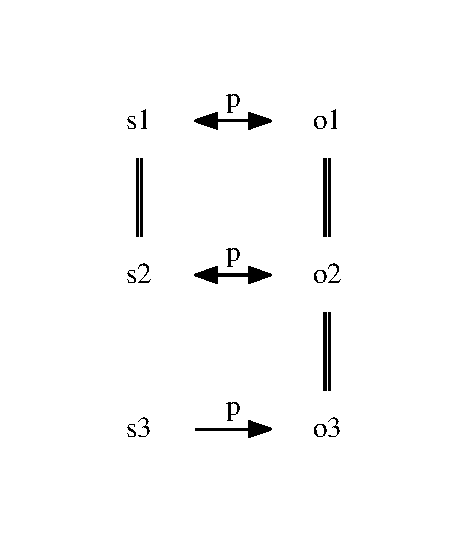
\includegraphics{./img/fixpoint_example}%[width=\columnwidth]
\caption{
  An illustrative example showing that defining
  $\underline{\approx}$ in terms of $\indp_{\approx}$ may not be optimal.
}
\end{figure}

The identity relation (equation \ref{eq:10}) is represented
  with double-lined edges in figure \ref{fig:example}.

\begin{equation}
\label{eq:10}
\approx = \set{\pair{s_1}{s_2},\pair{o_1}{o_2},\pair{o_2}{o_3}}
\end{equation}



\section{Calculating the lower approximation: Naive method}
\label{sec:naive}

The indiscernibility criteria for this example are as follows:

\begin{align}
\label{eq:20}
  \indp_{\approx}(\set{s_1,s_2,s_3})
=
  \indp_{\approx}(\set{o_1,o_2})
=
  \setdef{p^n}{\natnum{n}}
\end{align}

Based on the indiscernibility criteria in \ref{eq:20} and
  the definition of the lower approximation
  (def. \ref{def:lower_approximation1})
  we derive that the lower approximation is empty.



\section{Calculating the lower approximation: Fixpoint method}
\label{sec:fixpoint}

We now alter the definition of the lower approximation a bit,
  changing only the relation that is used for
  calculating the closures of the predicate and object terms
  in the specification of the discernibility criteria.
The resulting definition is \ref{def:lower_approximation2}.

\begin{definition}
\begin{align}
\label{def:lower_approximation2}
  x_1 \lowerapprox x_2
\, \iff \,\\
  \forall_{\pair{y_1}{y_2} \in S_G^2}(
        \indp_{\lowerapprox}(\set{y_1,y_2})
      =
        \indp_{\lowerapprox}(\set{x_1,x_2})
    \rightarrow
      y_1 \approx y_2
  )\nonumber
\end{align}
\end{definition}

Now there are two consistent solutions for the lower approximation:

\begin{enumerate}
\item $\lowerapprox_1 = \emptyset$,
      with $\indp_{\lowerapprox_1}(X) = \emptyset$
      for $X$ such that $\card{X} > 1$.
\item $\lowerapprox_2 = \set{\pair{s_1}{s_2},\pair{o_1}{o_2}}$,
      with $\indp_{\lowerapprox_2}(\set{s_1,s_2,o_1,o_2}) = \setdef{p^n}{\natnum{n}}$
      and $\indp_{\lowerapprox_1}(X) = \emptyset$
      for all other $X$ such that $\card{X} > 1$.
\end{enumerate}

The second solution seems to be the greatest correct solution here.
Both solutions are consistent/correct,
  since both conform to the same strictures imposed by the framework.
Since the lower approximation characterizes the pairs
  whose indiscernibility criteria are applied consistantly,
  it may also be reasonable from the application perspective to
  consider a greater lower approximation as more optimal
  (and the greatest lower approximation as most optimal).

\section{Higher approximation}

We have given an example for the lower approximation.
We expect that similar considerations apply to the higher approximation,
  where we maintain that the smallest higher approximation is
  the most optimal one.

\section{Appendix A: Generalized properties}

In the example from section \ref{sec:example} we have used
  properties denoted by \emph{sequences} of RDF predicate terms.
Definition \ref{def:indiscernibility_criteria} only deals with properties
  denoted by a single RDF predicate term.
Definition \ref{def:generalized_indiscernibility_criteria}
  provides the required generalization,
  using the functional mapping
  defined in \ref{def:generalized_property_map}.

\small
\begin{definition}[Generalized property map]
\begin{align}
\label{def:generalized_property_map}
  f_{\tuple{\range{p_1}{p_n}}}(s)
\,=\,
  \bigsetdef{o \in O_G}{
    \exists_{\range{x_0}{x_n}}(
      x_0 = s \land x_n = o \land\nonumber\\
      \bigwedge_{i=0}^{n-1}\nolimits
          \pair{I(x_i)}{I(x_{i+1})}
        \in
          \bigcup_{p \in \equivset{p_{i+1}}}\nolimits \mathit{Ext}(I(p))
    )
  }\nonumber
\end{align}
\end{definition}
\normalsize

\small
\begin{definition}[Generalized indiscernibility criteria]
\label{def:generalized_indiscernibility_criteria}
\begin{align}
  \indp_{\approx}(\set{\range{x_1}{x_n}})
=
  \setdef{
    \tuplerange{p_1}{p_n} \in P_G^n
  }{\\
      \exists_{\range{p_{11}}{p_{1n}} \in \equivset{p_1}},
    \ldots,
      \exists_{\range{p_{m1}}{p_{mn}} \in \equivset{p_n}}
    (\nonumber\\
        \equivset{f_{\tuplerange{p_{11}}{p_{m1}}} (x_1)}
      =
        \ldots
      =
        \equivset{f_{\tuplerange{p_{1n}}{p_{mn}}} (x_n)}
    )
  }\nonumber
\end{align}
\end{definition}
\normalsize

\end{document}

